% Copyright 2026 Sreeram Anil
% SPDX-License-Identifier: CC-BY-4.0
% =============================================================================
%  Federated (information-sharing) pack filter — pack-level family
% =============================================================================
\chapter{Federated Pack Filter (Federated)}
\label{ch:federated}

\section*{At a glance}
\begin{tabular}{@{}l>{\raggedright\arraybackslash}p{0.76\textwidth}@{}}
Family & pack-level (common state + per-cell deviation), decentralised \\
Header & \texttt{include/estkit/pack/federated.hpp} \\
Registered name & \texttt{Federated} \\
Structure & $N_c$ local EKFs on the common $\bar{\vx}\in\real^4$ + one master fusion \\
Information sharing & $\beta_j = 1/N_c$, $\sum_j\beta_j=1$; fusion-reset (FR) mode \\
Cost per step & \SI{5684}{\nano\second} for all $N_c=12$ nodes (\SI{474}{\nano\second} per node) \\
Memory & \SI{53472}{\byte} total (\SI{4336}{\byte} per node) \\
Bus load & 183 numbers per sample at every-step fusion; 20 at \SI{1}{\hertz} \\
Primary references & \cite{carlson1990federated,carlson1994federatedsim,carlson1988plans,mutambara1998} \\
\end{tabular}

\section{Motivation and aerospace/BMS relevance}
The centralised fusion of Chapter~\ref{ch:infofusion} is optimal but structurally fragile: one
node must receive every cell voltage every sample, and if it stops, the pack has no SOC at all.
Integrated navigation faced the identical problem in the 1980s --- a single Kalman filter fusing
INS, GPS, Doppler and TACAN is optimal but is a single point of failure and cannot be
certified sensor-by-sensor --- and Carlson's answer, the \emph{federated
filter} \cite{carlson1988plans,carlson1990federated}, became the standard architecture of
fault-tolerant navigation systems. It is the architecture this chapter transplants into a battery
module.

The battery version maps cleanly. Each cell-monitor slave holds a \emph{local filter} on the
common state $\bar{\vx}$, driven by the one voltage channel it owns, and a \emph{master} combines
the local estimates. Each slave therefore produces a complete, independently usable SOC estimate;
losing a slave removes one term from a sum. The BMS gets graceful degradation, per-channel fault
detection (each local filter has its own innovation sequence to monitor), and a bus that carries
$n_x + n_x(n_x{+}1)/2 = 14$ numbers per node per fusion instead of raw measurements at the
sampling rate.

None of this would be worth anything if the price were a badly suboptimal estimate. The remarkable
content of Carlson's construction is that, with the right \emph{information-sharing} factors, the
federated filter is not an approximation at all: it reproduces the centralised estimate exactly.
This chapter derives why, and the benchmark confirms it to four decimal places.

\section{Problem statement and assumptions}
Plant and notation as in Chapters~\ref{ch:bardelta} and \ref{ch:infofusion}: common state
$\bar{\vx}_k\in\real^{n_x}$, $n_x=4$, shared current $i_k$, per-cell measurements
\eqref{eq:if-meas} with the consider-noise treatment \eqref{eq:if-Rj} of the deviations.

\begin{assumption}[Common process, local measurements]\label{as:fed-common}
All $N_c$ local filters propagate the \emph{same} dynamics $f(\cdot),\mQ$ --- they are $N_c$
filters on one state, not $N_c$ filters on $N_c$ states --- and their measurement noises are
mutually independent (Assumption~\ref{as:if-indep}).
\end{assumption}
\begin{assumption}[Correlation through the shared process noise]\label{as:fed-corr}
Because they share $\mQ$, the errors of the local estimates are \emph{correlated} even when the
measurement noises are not. Simply summing local information would therefore count the common
process noise $N_c$ times and produce an optimistic (inconsistent) covariance. Removing that
double counting is what information sharing does.
\end{assumption}

\section{Derivation}

\subsection{The information-sharing principle}
Write the centralised filter's prior information at time $k$ as
$\bm{Y}^-_k=(\Pminus_k)\inv$. Assign to local filter $j$ a share $\beta_j$ of the common
information, i.e.\ give it the \emph{deflated} prior and process noise
\begin{equation}
\boxed{\;\mP_{j}(0) = \frac{\mP(0)}{\beta_j},\qquad \mQ_j = \frac{\mQ}{\beta_j},\qquad
\sum_{j=1}^{N_c}\beta_j = 1,\ \beta_j>0.\;}
\label{eq:fed-share}
\end{equation}
Each local filter is now \emph{conservative}: it believes it knows $1/\beta_j$ times less than the
centralised filter does. The master recombines the local estimates by the standard
maximum-likelihood (information) fusion of independent estimates,
\begin{equation}
\mP_m\inv = \sum_{j=1}^{N_c}\mP_j\inv ,\qquad
\vx_m = \mP_m\sum_{j=1}^{N_c}\mP_j\inv\vx_j .
\label{eq:fed-fuse}
\end{equation}

\begin{theorem}[Carlson, 1990 \cite{carlson1990federated}]\label{thm:fed}
Let the local filters satisfy Assumption~\ref{as:fed-common}, let their priors and process noises
be deflated by \eqref{eq:fed-share} with $\sum_j\beta_j=1$, and let them be re-initialised after
each fusion with
\begin{equation}
\vx_j \leftarrow \vx_m,\qquad \mP_j\leftarrow \mP_m/\beta_j \qquad\text{(fusion-reset, FR)} .
\label{eq:fed-reset}
\end{equation}
Then $(\vx_m,\mP_m)$ of \eqref{eq:fed-fuse} equals the centralised estimate
$(\bar{\vx}^+_k,\Pplus_k)$ of \eqref{eq:if-Y}--\eqref{eq:if-x} exactly, at every fusion epoch.
\end{theorem}

\begin{proof}[Proof for the linear case, one cycle]
Let $\mP_c^-$ be the centralised prior and suppose the reset \eqref{eq:fed-reset} has just left
$\mP_j^+ = \mP_c^+/\beta_j$ and $\vx_j=\vx_c$ for all $j$. Propagating local filter $j$ with the
deflated process noise,
\begin{equation}
\mP_j^- = \mF\frac{\mP_c^+}{\beta_j}\mF^\T + \frac{\mQ}{\beta_j}
        = \frac{1}{\beta_j}\big(\mF\mP_c^+\mF^\T+\mQ\big) = \frac{\mP_c^-}{\beta_j},
\label{eq:fed-proof1}
\end{equation}
so the deflation is \emph{invariant} under the time update --- this is the step that requires
$\mQ_j=\mQ/\beta_j$ and not merely a deflated prior. The local measurement update in information
form gives
\begin{equation}
\big(\mP_j^+\big)\inv = \big(\mP_j^-\big)\inv + \mH_j^\T R_j\inv\mH_j
 = \beta_j\big(\mP_c^-\big)\inv + \mH_j^\T R_j\inv\mH_j .
\label{eq:fed-proof2}
\end{equation}
Summing over $j$ and using $\sum_j\beta_j=1$,
\begin{equation}
\sum_{j}\big(\mP_j^+\big)\inv = \Big(\sum_j\beta_j\Big)\big(\mP_c^-\big)\inv + \sum_j \mH_j^\T R_j\inv\mH_j
 = \big(\mP_c^-\big)\inv + \sum_j\mH_j^\T R_j\inv\mH_j = \big(\mP_c^+\big)\inv,
\label{eq:fed-proof3}
\end{equation}
which is exactly \eqref{eq:if-Y}: the master covariance is the centralised covariance. For the
mean, all locals start the cycle at $\vx_j^+=\vx_c$ and share $f$, so $\vx_j^-=\vx_c^-$ for every
$j$, and the local information-vector updates are
\begin{equation}
\big(\mP_j^+\big)\inv\vx_j^+ = \big(\mP_j^-\big)\inv\vx_j^- + \mH_j^\T R_j\inv\tilde y_j
 = \beta_j\big(\mP_c^-\big)\inv\vx_c^- + \mH_j^\T R_j\inv\tilde y_j ,
\label{eq:fed-proof4}
\end{equation}
with $\tilde y_j = v_j - h(\vx_c^-,\vu_j) + \mH_j\vx_c^-$ the linearised measurement referred to
the origin. Summing \eqref{eq:fed-proof4} over $j$ and using $\sum_j\beta_j=1$ again,
\begin{equation}
\sum_j\big(\mP_j^+\big)\inv\vx_j^+ = \big(\mP_c^-\big)\inv\vx_c^- + \sum_j\mH_j^\T R_j\inv\tilde y_j
 = \big(\mP_c^+\big)\inv\vx_c^+ ,
\label{eq:fed-proof5}
\end{equation}
so $\vx_m = \mP_m\sum_j(\mP_j^+)\inv\vx_j^+ = \mP_c^+\big(\mP_c^+\big)\inv\vx_c^+ = \vx_c^+$.
\end{proof}

The proof makes the role of $\sum_j\beta_j = 1$ transparent: it is a conservation law for
information. If $\sum_j\beta_j>1$ the prior is counted more than once and the fused covariance is
too small (the filter becomes over-confident and eventually diverges); if $\sum_j\beta_j<1$ prior
information is thrown away and the estimate is merely conservative. The benchmark exhibits both
effects: setting $\beta_j=1/2$ (so $\sum_j\beta_j=6$) degrades \texttt{nominal} rmse from
\num{0.0055} to \num{0.0109} and \texttt{large\_imbalance} from \num{0.0094} to \num{0.0299}.

\subsection{Reset modes}
Theorem~\ref{thm:fed} needs the reset \eqref{eq:fed-reset}, because \eqref{eq:fed-proof1} assumes
the locals start the cycle deflated by exactly $\beta_j$. Carlson's taxonomy
\cite[Tab.~I]{carlson1990federated} also allows:
\begin{itemize}[nosep]
\item \textbf{FR} (fusion reset, implemented default): \eqref{eq:fed-reset}; optimal, but the
      master must broadcast $(\vx_m,\mP_m)$ back to every node.
\item \textbf{NR} (no reset): locals keep their own estimates and are never corrected; the master
      output \eqref{eq:fed-fuse} is still consistent but strictly conservative, and no downlink
      is needed. Measured penalty: \texttt{nominal} rmse \num{0.0064} against \num{0.0055}.
\item \textbf{ZR} (zero reset): locals are reset to zero information and the master holds all of
      it; maximum fault isolation, largest accuracy penalty. Not implemented here.
\end{itemize}
Fusion need not happen every sample. The implementation exposes \texttt{fuse\_every}; between
fusions the master dead-reckons its mean through the model, $\vx_m\leftarrow f(\vx_m,\bar{\vu})$,
which is exactly what a federated master with $\beta_m=0$ (no measurements of its own) does.

\subsection{The nonlinear and battery-specific parts}
Three things change relative to Carlson's linear derivation.

\emph{(i) Linearisation point.} Each local filter linearises $f$ and $h$ at its own estimate. In
FR mode with every-step fusion all locals start from $\vx_m$, so the linearisation points
coincide and Theorem~\ref{thm:fed} survives the nonlinearity exactly; with \texttt{fuse\_every}
$>1$ or in NR mode they drift apart and the equality becomes an approximation.

\emph{(ii) Local measurement noise.} Local filter $j$ sees its own cell, not the average, so its
measurement carries the deviation $\delta_j$ of \eqref{eq:if-meas}. It is accounted for by the
inflation \eqref{eq:if-Rj},
\begin{equation}
R_j = \sigma_v^2 + \big(\bar R_0\sigma_i\big)^2 + \big(\ocv'(\bar\soc)\sigma_{\Delta\soc}\big)^2 + \big(\epsilon_R w^{\mathrm{tot}}\big)^2 ,
\label{eq:fed-Rj}
\end{equation}
and by subtracting the already-identified part $\hat\delta_j$ from $v_j$ before the update
(\texttt{compensate\_deviation}, worth \num{0.0055} against \num{0.0060} on \texttt{nominal}).
Because $\sum_j\Delta\hat\soc_j=0$, the compensation is zero-mean over the module and cannot bias
$\vx_m$.

\emph{(iii) Per-cell output.} As in the rest of the family, $\hat\soc_j = \hat{\bar\soc}_m +
\Delta\hat\soc_j$ with the 3-state delta filters of Chapter~\ref{ch:bardelta}, driven by the
\emph{local} residual $v_j - h(\vx_m,\vu_j)$, which needs no communication beyond the $\vx_m$
that FR mode already broadcasts.

\section{Algorithm}
\begin{algorithm}[H]
\caption{Federated (FR mode) --- one sampling period $k$}
\begin{algorithmic}[1]
\Require local $\{\vx_j,\mP_j\}$ with $\mQ_j = \mQ/\beta_j$, delta states $\{\bm{d}_j\}$, $i_k$, $\{v_{j,k}\},\{T_{j,k}\}$
\ForAll{nodes $j = 1,\dots,N_c$ \textbf{in parallel}}
  \State $\vu_j\gets[i_k,T_{j,k}]^\T$;\;
         $\vx_j\gets f(\vx_j,\vu_j^{k-1})$;\; $\mP_j\gets\mF\mP_j\mF^\T+\mQ/\beta_j$
  \State $R_j$ from \eqref{eq:fed-Rj};\;
         local EKF update with $y = v_{j,k}-\hat\delta_j$
  \State send $(\vx_j,\mP_j)$ to the master \Comment{$n_x + n_x(n_x{+}1)/2 = 14$ numbers}
\EndFor
\If{$k \bmod \texttt{fuse\_every} = 0$}
  \State \textbf{master:} $\bm{Y}\gets\sum_j\mP_j\inv$;\;
         $\mP_m\gets\bm{Y}\inv$;\; $\vx_m\gets\mP_m\sum_j\mP_j\inv\vx_j$ \hfill \eqref{eq:fed-fuse}
  \State broadcast $(\vx_m,\mP_m)$;\quad
         \textbf{each node:} $\vx_j\gets\vx_m$, $\mP_j\gets\mP_m/\beta_j$ \hfill \eqref{eq:fed-reset}
\Else
  \State \textbf{master:} $\vx_m\gets f(\vx_m,\bar{\vu}_k)$ \Comment{dead reckoning between fusions}
\EndIf
\State \textbf{Delta layer} (every $r$ samples): update $\{\bm{d}_j\}$ from $v_{j,k}-h(\vx_m,\vu_j)$
\Ensure $\hat\soc_{j,k}=\hat{\bar\soc}_m + \Delta\hat\soc_{j,k}$
\end{algorithmic}
\end{algorithm}

\section{Application to the battery model}
\texttt{FederatedPack<Filter,Model>} is a template over the local filter type; the registered
estimator uses \texttt{Ekf<EcmModel>}, and the information deflation $\mQ_j=\mQ/\beta_j$ is
applied through the filter's own \texttt{opts.q\_scale} (detected at compile time with a
\texttt{void\_t} trait, so a filter without that knob still compiles). $\mP_j(0)=\mP_0/\beta_j$ is
applied at \texttt{init()}, and the reset \eqref{eq:fed-reset} through \texttt{x\_mut()} and
\texttt{P\_mut()}. The measurement-noise inflation \eqref{eq:fed-Rj} is realised by writing the
effective $\sigma_v$ into the local filter's own model copy each step, so the generic
\texttt{Ekf} needs no modification. Running the same class with \texttt{Ukf<EcmModel>} works but
is worse (\texttt{nominal} rmse \num{0.0261} at \SI{11936}{\nano\second}/step): with $\mQ$
inflated twelve-fold the sigma points span a large prior and the subtractive UKF covariance update
loses accuracy, so the EKF is the better local filter here.

Defaults: $\beta_j=1/N_c$ (equal sensors), \texttt{fusion\_reset = true},
\texttt{fuse\_every = 1}, $\sigma_{\Delta\soc}=\num{0.03}$, $\epsilon_R=\num{0.08}$,
\texttt{compensate\_deviation = true}.

\section{Implementation notes}
Storage is a \texttt{std::array<Filter, kPackCells>} built once from a prototype (filters have no
default constructor), so no heap is touched after construction and the per-node objects are
contiguous. The fusion loop performs $N_c$ $4\times4$ inversions and one more for $\mP_m$; each is
checked with \texttt{is\_finite()} and the entire fusion is skipped --- leaving the locals
untouched --- if any node's covariance is singular, so a failed node cannot corrupt the master.
$\bm{Y}$ and $\mP_m$ are symmetrised, and $\vx_m$ is projected onto the physical set
($\soc\in[-0.05,1.05]$, $|h|\le1$).

\emph{Communication accounting.} \texttt{messages\_per\_step()} counts the scalars that cross the
module bus per sample, each broadcast counted once:
$N_c(n_x + n_x(n_x{+}1)/2)/\texttt{fuse\_every}$ uplink, plus $(n_x+n_x(n_x{+}1)/2)$ downlink in FR
mode, plus $(N_c+1)/r$ for the zero-mean projection of the delta layer. With the defaults this is
$12\times14 + 14 + 13/10 = 183$ numbers per sample, against \num{12} for the centralised fusion
--- the federated architecture trades \num{15} times the bus load for the removal of the single
point of failure. Sending the Cholesky factor or the information pair $(\bm{Y}_j,\bm{Y}_j\vx_j)$
instead does not change the count; sending $\mP_j$ only at fusion epochs does, which is what
\texttt{fuse\_every} controls.

\emph{Cost.} \SI{5684}{\nano\second} per sample for the whole module, i.e.\ \SI{474}{\nano\second}
per node --- but these $N_c$ nodes run \emph{concurrently} on $N_c$ processors in the intended
architecture, so the wall-clock cost per node is that of one cell-level EKF plus $1/N_c$ of one
fusion. The benchmark executes them sequentially on one core, which is why the total exceeds the
decentralised baseline; the meaningful comparison is per-node. Memory is
$N_c\times\SI{4336}{\byte}=\SI{52}{\kibi\byte}$, of which $N_c\times\SI{3872}{\byte}$ is $N_c$
private copies of the OCV table --- in a real system one shared read-only table, leaving
\SI{464}{\byte} of RAM per node.

\emph{Limitations.} (i) Theorem~\ref{thm:fed} needs Assumption~\ref{as:fed-common}; if the local
filters had different dynamics (different capacities per cell, say) the deflation would no longer
commute with the time update and the equality becomes approximate. (ii) In FR mode a corrupted
master corrupts every node at the next reset; NR mode is the fault-tolerant choice and costs
\SI{16}{\percent} accuracy. (iii) The master's dead reckoning between fusions is open loop, which
is what produces the large transient of the slow-fusion variants below.

\section{Benchmark results}
% Copyright 2026 Sreeram Anil
% SPDX-License-Identifier: CC-BY-4.0
\begin{table}[H]\centering\footnotesize\setlength{\tabcolsep}{4pt}\caption{Federated: pack-level benchmark (12-cell module, eVTOL mission, mean over seeds; all errors in \% SOC). RMSE$_\mathrm{cells}$: per-cell RMSE over all cells; RMSE$_{\min/\mathrm{mean}/\max}$: error of the weakest / mean / strongest-cell SOC; 53472 bytes of state, 183 numbers exchanged per step.}\label{tab:pack_Federated}
\begin{tabular}{lrrrrrrcr}\toprule scenario & RMSE$_\mathrm{cells}$ & RMSE$_{\min}$ & RMSE$_\mathrm{mean}$ & RMSE$_{\max}$ & max cell err. & RMSE$_\mathrm{ss}$ & div. & ns/step \\ \midrule
nominal & 0.55 & 0.48 & 0.38 & 0.46 & 3.09 & 0.56 & no & 8346 \\
init\_error & 0.54 & 0.44 & 0.37 & 0.46 & 2.67 & 0.57 & no & 8320 \\
current\_bias & 0.84 & 0.91 & 0.75 & 0.82 & 3.46 & 0.92 & no & 8448 \\
weak\_cell & 0.57 & 0.51 & 0.37 & 0.61 & 3.00 & 0.53 & no & 8368 \\
noise\_step & 0.56 & 0.51 & 0.38 & 0.45 & 3.09 & 0.59 & no & 8275 \\
large\_imbalance & 0.94 & 1.65 & 0.66 & 0.64 & 9.40 & 0.71 & no & 8379 \\
\bottomrule\end{tabular}\end{table}

\begin{figure}[H]\centering
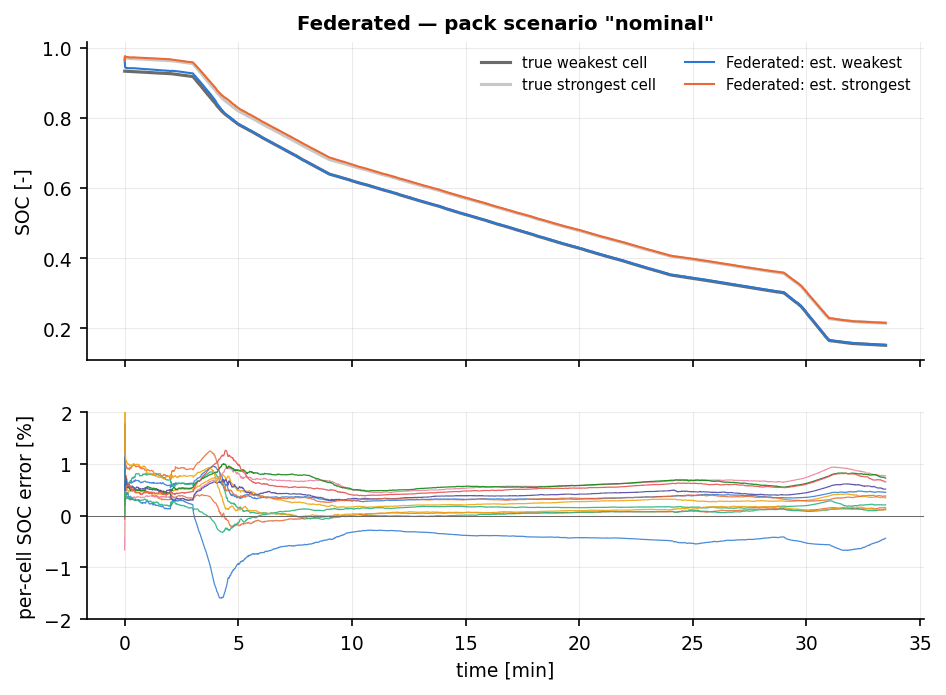
\includegraphics[width=\textwidth]{figures/pack_Federated_nominal.png}
\caption{Federated on the nominal eVTOL mission: per-cell SOC, min/mean/max envelope and error.}
\end{figure}
\begin{figure}[H]\centering
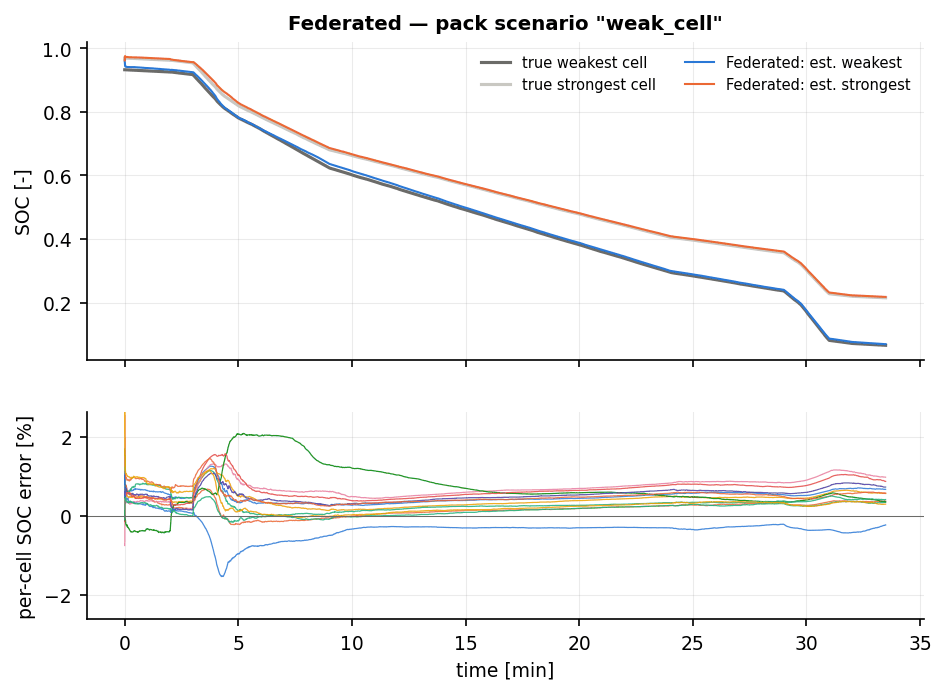
\includegraphics[width=\textwidth]{figures/pack_Federated_weak_cell.png}
\caption{Federated on \texttt{weak\_cell}: node 5 owns the aged cell; its inflated $R_j$ and the
fusion \eqref{eq:fed-fuse} keep the common state clean while the local delta filter tracks the
divergence.}
\end{figure}

\begin{center}\small
\begin{tabular}{@{}lcccc|cccc@{}}
\toprule
& \multicolumn{4}{c|}{\estname{Federated}} & \multicolumn{4}{c}{\estname{Decentralized-EKF}} \\
Scenario & rmse & rmse$_{\min}$ & ss & max & rmse & rmse$_{\min}$ & ss & max \\
\midrule
\texttt{nominal}          & 0.0055 & 0.0048 & 0.0056 & 0.031 & 0.0123 & 0.0081 & 0.0134 & 0.046 \\
\texttt{init\_error}      & 0.0054 & 0.0044 & 0.0057 & 0.027 & 0.0118 & 0.0082 & 0.0129 & 0.042 \\
\texttt{current\_bias}    & 0.0084 & 0.0091 & 0.0092 & 0.035 & 0.0137 & 0.0088 & 0.0148 & 0.056 \\
\texttt{weak\_cell}       & 0.0057 & 0.0051 & 0.0053 & 0.030 & 0.0129 & 0.0129 & 0.0137 & 0.048 \\
\texttt{noise\_step}      & 0.0056 & 0.0051 & 0.0059 & 0.031 & 0.0122 & 0.0084 & 0.0131 & 0.045 \\
\texttt{large\_imbalance} & 0.0094 & 0.0165 & 0.0071 & 0.094 & 0.0174 & 0.0245 & 0.0179 & 0.061 \\
\midrule
\si{\nano\second}/step & \multicolumn{4}{c|}{5684 (474/node)} & \multicolumn{4}{c}{3860 (322/node)} \\
bytes & \multicolumn{4}{c|}{53472} & \multicolumn{4}{c}{52032} \\
messages/step & \multicolumn{4}{c|}{183} & \multicolumn{4}{c}{0} \\
\bottomrule
\end{tabular}
\end{center}
(Means over three seeds; \texttt{rmse$_{\min}$} is the error of the reported weakest-cell SOC.)

\paragraph{Theorem~\ref{thm:fed} is confirmed numerically.} Across all six scenarios and three
seeds the \estname{Federated} and \estname{InfoFusion} rows agree to every printed digit
($\num{0.0055}$, $\num{0.0054}$, $\num{0.0084}$, $\num{0.0057}$, $\num{0.0056}$,
$\num{0.0094}$); the residual
differences appear only in the fifth significant figure and come from the different arithmetic
paths ($N_c$ small inversions and one fusion versus one accumulation of rank-one terms). This is
the strongest statement the benchmark can make about information sharing: the federated filter
buys \emph{distribution and fault tolerance for free in accuracy}, and pays only in bus load
(\num{183} versus \num{12} numbers per sample) and, on a single processor, in arithmetic
(\SI{5684}{\nano\second} versus \SI{1463}{\nano\second} for the whole module on one core).

\paragraph{The cost of the architectural choices.} One paired run over two seeds, so that every
variant sees identical data (the default row therefore differs in the last digit from the
three-seed table above):
\begin{center}\small
\begin{tabular}{@{}lccccr@{}}
\toprule
Variant & \texttt{nominal} & \texttt{weak\_cell} & \texttt{large\_imb.} & \texttt{init\_error} max & messages/step \\
\midrule
FR, fuse every sample (default) & 0.0055 & 0.0057 & 0.0094 & 0.027 & 183 \\
FR, fuse at \SI{1}{\hertz}              & 0.0063 & 0.0066 & 0.0173 & 0.367 &  20 \\
FR, fuse at \SI{0.1}{\hertz}            & 0.0069 & 0.0070 & 0.0177 & 0.378 &   3 \\
NR (no reset)                   & 0.0064 & 0.0068 & 0.0164 & 0.037 & 170 \\
$\beta_j=1/2$ ($\sum\beta_j=6$) & 0.0109 & 0.0145 & 0.0299 & 0.076 & 183 \\
no deviation compensation       & 0.0060 & 0.0064 & 0.0131 & 0.027 & 183 \\
\bottomrule
\end{tabular}
\end{center}
Fusing at \SI{1}{\hertz} instead of \SI{10}{\hertz} cuts the bus load by a factor \num{9} and
costs \SI{15}{\percent} of steady-state accuracy --- an excellent trade for a CAN-based module
--- but the \texttt{init\_error} column exposes the catch: between fusions the master dead-reckons,
so during the first convergence from a \SI{35}{\percent} SOC error the reported estimate lags by
up to \num{0.367} for up to \texttt{fuse\_every} samples. A practical design fuses fast while the
master covariance is large and slows down once it has converged. The $\beta_j=1/2$ row is the
experimental counterpart of the conservation law $\sum_j\beta_j=1$: with six times too much
information the fused covariance is optimistic and the error doubles, without ever formally
diverging. NR mode costs \SI{16}{\percent} accuracy and removes the downlink; it is the mode to
choose when a corrupted master must not be able to poison the slaves.

\paragraph{Against the decentralised baseline.} \estname{Federated} halves the error of
\estname{Decentralized-EKF} in every scenario (\num{0.0055} versus \num{0.0123} on
\texttt{nominal}, \num{0.0051} versus \num{0.0129} on the safety-critical weakest-cell metric in
\texttt{weak\_cell}) using \emph{the same number of processors and the same number of filters},
differing only in that they estimate a shared state and exchange 14 numbers per node. The
per-node arithmetic is comparable (\SI{474}{\nano\second} against \SI{322}{\nano\second}: one
$4\times4$ EKF in both cases, plus a share of the fusion). This is the clearest statement of what
information sharing is worth in a pack: at essentially the cost of the naive decentralised
architecture, it delivers the centralised optimum.

\section{Summary}
Use the federated filter when the pack architecture is genuinely distributed --- one processor per
module or per cell group --- and single-point-of-failure behaviour is unacceptable, which in an
aircraft battery it usually is. Deflate both the prior \emph{and} the process noise by
$\beta_j=1/N_c$, check that $\sum_j\beta_j=1$, and use fusion-reset if you want the centralised
optimum or no-reset if you want fault isolation; the measured difference is \SI{16}{\percent}.
Fuse as often as the bus allows, and fuse fast during transients. Do not use it when all the data
already arrive at one node anyway (then Chapter~\ref{ch:infofusion} gives the same answer at one
quarter of the arithmetic and one fifteenth of the traffic), and do not use it with local filters
whose dynamics differ --- the equality of Theorem~\ref{thm:fed} rests on a common process model.
